%\documentclass[times, 10pt, twocolumn]{article} 
%\documentclass[conference,final]{IEEEtran}
     
\documentclass{rspublic}   

%\usepackage{latex8}
%\usepackage{times}

%\documentstyle[times,art10,twocolumn,latex8]{article}

%------------------------------------------------------------------------- 
% take the % away on next line to produce the final camera-ready version 
%\pagestyle{empty}

\usepackage[utf8]{inputenc}
\usepackage{graphicx}
\usepackage{url}
\usepackage{float}
\usepackage{times}    
\usepackage{multirow}    
\usepackage{listings}   
\usepackage{times}     
\usepackage{paralist}    
\usepackage{wrapfig}    
\usepackage[small,it]{caption}
\usepackage{multirow}
\usepackage{ifpdf}    
\usepackage{subfig} 
                    
%Bibliography                     
\usepackage{natbib}   

\usepackage{listings}
\usepackage{keyval}  
\usepackage{color}
\definecolor{listinggray}{gray}{0.95}
\definecolor{darkgray}{gray}{0.7}
\definecolor{commentgreen}{rgb}{0, 0.4, 0}
\definecolor{darkblue}{rgb}{0, 0, 0.4}
\definecolor{middleblue}{rgb}{0, 0, 0.7}
\definecolor{darkred}{rgb}{0.4, 0, 0}
\definecolor{brown}{rgb}{0.5, 0.5, 0}

\lstdefinestyle{myListing}{
  frame=single,   
  backgroundcolor=\color{listinggray},  
  %float=t,
  language=C,       
  basicstyle=\ttfamily \footnotesize,
  breakautoindent=true,
  breaklines=true
  tabsize=2,
  captionpos=b,  
  aboveskip=0em,
  %numbers=left, 
  %numberstyle=\tiny
}      

\lstdefinestyle{myPythonListing}{
  frame=single,   
  backgroundcolor=\color{listinggray},  
  %float=t,
  language=Python,       
  basicstyle=\ttfamily \footnotesize,
  breakautoindent=true,
  breaklines=true
  tabsize=2,
  captionpos=b,  
  %numbers=left, 
  %numberstyle=\tiny
}


\title[Distributed Replica-Exchange Simulations]{Distributed
  Replica-Exchange Simulations}

% \title[Distributed Replica-Exchange Simulations]{ Distributed
%   Replica-Exchange Simulations on Production Environments using SAGA
%   and Migol}

% \title{Reliable Replica-Exchange Simulations of Biomolecular Systems
%   on Production Distributed Environments using SAGA-CPR and Migol}
% Computational Grids using SAGA-CPR and Migol}


\author[Luckow, Jha, Kim, Merzky, Schnor]{
  Andr\'e Luckow$^{1}$, Shantenu Jha$^{2,3,4}$, Joohyun Kim$^{2}$, Andre Merzky$^{2}$ and Bettina Schnor$^{1}$\\
  \small{\emph{$^{1}$Institute of Computer Science, Potsdam University, Germany}}\\
  \small{\emph{$^{2}$Center for Computation \& Technology, Louisiana State University, USA}}\\
  \small{\emph{$^{3}$Department of Computer Science, Louisiana State
      University, USA}}\\
  \small{\emph{$^{4}$e-Science Institute, Edinburgh, UK}}\\
}

%\date{}

\def\acknowledgementname{Acknowledgements}
\newenvironment{acknowledgement}%
{\section*{\acknowledgementname}%
\parindent=0pt%
}

\newif\ifdraft
\drafttrue
\ifdraft
\newcommand{\kimnote}[1]{ {\textcolor{green} { ***JK: #1 }}}
\newcommand{\alnote}[1]{ {\textcolor{blue} { ***AL: #1 }}}
\newcommand{\amnote}[1]{ {\textcolor{magenta} { ***AM: #1 }}}
\newcommand{\jhanote}[1]{ {\textcolor{red} { ***SJ: #1 }}}
\else
\newcommand{\kimnote}[1]{}
\newcommand{\alnote}[1]{}
\newcommand{\amnote}[1]{}
\newcommand{\jhanote}[1]{}
\fi

\newcommand{\glidein}[1]{Glide-In }  
\newcommand{\replicaagent}[1]{Replica-Agent }

\begin{document} 


\maketitle    

\begin{abstract}{REMD, SAGA, Migol, Fault Tolerance}  
  There exists a class of scientific applications for which utilizing
  distributed resources is critical for reducing the
  time-to-solution. However, the ability to orchestrate many
  distributed jobs in a distributed environments is a major challenge.
  We discuss a specific class of applications -- Replica-Exchange
  simulations -- where utilizing as many (often heterogenous)
  distributed resources as possible, is critical for the effective
  solution of the scientific problem.  SAGA is a high-level
  programmatic abstraction layer that provides a standardised
  interface for the primary distributed functionality required for
  application development.

  \jhanote{In this paper, we describe the design, development and
    deployment of a unique framework for constructing fault-tolerant
    distributed simulations.}

  \jhanote{Less emphasis on the SAGA/Migol framework: The framework
    consists of two primary components -- SAGA and Migol, is scalable,
    general purpose and extensible.}

  \jhanote{I think this can go: We provide details of a newly
    developed functionality in SAGA -- the Checkpoint and Recovery
    API. Migol is an adaptive Grid middleware, which addresses the
    fault tolerance of Grid applications and services by providing the
    capability to recover applications from checkpoint files
    transparently.  In addition to describing the integration of
    SAGA-CPR with the Migol infrastructure,}

  \jhanote{We also outline our experiences with running a large scale,
    general-purpose, SAGA-CPR based Replica-Exchange application in a
    production distributed environment.}

\end{abstract}

\section{Introduction}
                 
\begin{itemize}

\item The move of traditional algorithms to distributed systems holds
  the promise of reduced time-to-solution and other advantages, but
  comes with its own set of challenges. For example, there is a
  trading of control and comfort of a single environment, for the
  coordination hassles of distributed systems. In particular, the need
  to schedule multiple resources is challenging. The stringency of the
  requirement of scheduling resources changes with the level of
  application-level coupling. For example, for tightly-coupled
  MPICH-G2 style jobs, complete synchrony is required; for
  loosely-coupled applications/replicas there is still a need to
  co-schedule resources, but the choice of clever
  algoirthms/implementations can relax this requirement. In
  pathological cases, all systems can come to a grinding halt if a
  global synchronization of the different components is required
  between successive stages, and any one component has not even
  started!

\item There are different levels of Abstractions  that are required
  in order to make distributed systems generally more usable for
  production science. By one classification, the three levels of
  classification are, i) application level, ii) deployment iii) system-level
  level (usage) abstraction

\item A unique/novel contribution of this paper is the first
  implementation of a system-level abstraction (analogous to Glide-In)
  using programmatic interfaces, and a novel implementation of the
  replica-exchange algorithm to exploit resources opportunistically.
  However it is critical to point out that the {\it novel} RE
  implementation is practical only because of {\bf the agile execution
    model} that the programming model and system bestows! The
  generalization of the RE algorithm is trivial, but ensuring its
  implementation and execution isn't and {\bf depends critically upon
    SAGA and its enhanced job model.}

\item Algorithmic behaviour/constraints on a localized/single cluster
  can be very different for distributed clusters. Interesting to
  mention that it is trivial to port this framework onto a top-end
  machine such as Ranger that is pushing the limits of petascalabilty..

\end{itemize}
          
There exist several types of applications, which are well suited
to distributed environments. Probably the best known and most powerful
example are those that involve an ensemble of decoupled tasks, which
we refer to as {\it pleasingly-distributed} applications; in spite of
its conceptual simplicity, many scientific problems based on parameter
sweeps and/or Monte Carlo simulations, can be solved using
infrastructure that supports this common application class. A slightly
more complicated and challenging class of distributed applications are
those that have a small level of coupling between individual
sub-tasks.  An interesting example of such applications are those
based on \emph{Replica-Exchange (RE)}~\citep{hansmann,Sugita:1999rm}
simulations.  Such applications can be used to understand important
physical phenomena -- ranging from protein folding dynamics to binding
affinity calculations required for computational drug discovery.

Distributed RE simulations must be able to orchestrate different
heterogeneous resources in a complex and dynamic environment.  Writing
such applications is a complex task for a myriad number of reasons,
not least of which is that distributed computing environments are
inherently prone to failures and thus
unreliable~\citep{schroeder,10.1109/E-SCIENCE.2006.93,DBLP:conf/grid/KhaliliHOSC06}.
Some applications can respond to such failures via redundant or
speculative computing.  However, redundant computing has its
limitations, especially when there is a level of heterogeneity and
coupling between tasks.  Speculative computing is still possible, but
its use to mitigate the consequence of distributed failures, leads to
a whole host of load-balancing and scheduling problems.

Partly due to some of these challenges, even though distributed RE
simulations are loosely-coupled, failures can become a major problem
for such applications.  In RE simulations, there is a need to
occasionally attempt an exchange between pairs of replicas; the
pairing of replicas is not a constant but is dynamically evolving.
However, once a pair of replicas has been established, a delay or loss
of one replica will stall the other replica.  Thus over time, due to
the fact that in principle, every replica will ultimately
interact/exchange with another replica, a single failure, if left
uncorrected can ultimately cause the simulation to encounter an
exponentially increasing slow-down.  In the worst case, a single
failing task can render the entire computation worthless.  Thus, it is
essential to provide support for fault tolerance at some level.
\emph{Migol}~\citep{schnorLuckow08} provides fault-tolerance at the
middleware level by supporting the transparent starting, monitoring
and recovery of tasks.

\jhanote{there is repetition here. need to refine} \amnote{the last
  sentence reads strange to me.  What is the 'thus' referring to?  That
  migol provides fault tolerance?}      
\alnote{I reordered the sentences - should be ok now.}

Having motivated the need for a fault-tolerant framework for
application development, in particular for distributed RE simulations,
this paper describes the design of the SAGA~\citep{saga_gfd90}
Checkpoint\,\&\,Recovery package (CPR), and its implementation using
the Migol adaptor. SAGA-CPR~\citep{saga-cpr} represents the first
extension to the core SAGA API specification, and is thus a validation
of the extensibility of the specification.  Additionally Migol can be
regarded as a reference implementation of the GridCPR
architecture~\citep{ogf_cpr_arch}.  We demonstrate this by presenting
the seamless integration of CPR concepts and abstractions into the
SAGA framework; the resulting system is able to provide an easy to
use, high-level programming abstractions for Grid enabled, fault
tolerant applications.  The pairing of Migol and SAGA-CPR thus
provides a natural, portable and a very generic solution to the
problem of a programmatic interface for designing fault-tolerant
applications.  To highlight this and that it is critical that all
aspects of the distributed application life-cycle -- design,
development and deployment -- are made easier, we will discuss our
experiences in developing and deploying a RE application in a
production environment.


Before outlining the structure of the paper, we highlight the main
advantages of our approach: First and foremost it is a general purpose
framework that can be used over a wide-range of distributed production
environments, such as the TeraGrid, UK's NGS, DEISA, etc., as opposed
to WISDOM~\citep{wisdom}, that is essentially confined to
gLITE/EGEE. Secondly, our approach can scale to use resources of
different sizes, as opposed to {\it Folding@home}~\citep{folding} which
is based upon BOINC, and is thus inherently limited in the size of
physical problems that can be solved effectively.  \alnote{Should we
  add citations to Folding@home and wisdom here?}  Thirdly, our
framework is extensible: it can be used to implement many other
application in addition to those based upon RE
simulations~\citep{escience07}. The power to do so arises
from simple design decisions: the use of standard interfaces on the
one hand, and the use of appropriate programmatic and system
abstractions that allow users to do what they can do best
(i.e. provide the simulation and orchestration logic), whilst ensuring
that middleware used provides required services (such as checkpoint
management, application monitoring and recovery) seamlessly and
effectively from the application developers perspective.

The remainder of the paper is structured as follows: In the next
section we provide the basic ideas behind RE and specifically
Replica-Exchange using Molecular Dynamics simulations.  We then
discuss the SAGA CPR package and its relation to the  fault-tolerant 
Migol framework. In section 4 we present
the challenges of developing developing a REMD application, which is runnable in 
a heterogeneous and loosely coupled Grid environment.
In section 5, we discuss how SAGA and Migol are used to implement 
a fault-tolerant, distributed framework for RE. In the subsequent sections we discuss
our experience in implementing REMD and performance figures. We
conclude by providing a detailed analysis of related work, which will
highlight the truly unique features of our implementation.

\section{Replica-Exchange Molecular Dynamics}
\alnote{I restructured this section: 1) general introduction to MD
  problems and further motivation for RE algorithm 2)
  Structure/Classification of REMD algorithms}  In Molecular
Dynamics (MD) approaches, a sufficient sampling of configurations is
an important requirement for connecting atomistic results to
macroscopic or thermodynamic quantities available from experiments.
However, even with the most powerful computing resources at the
moment, straight-forward MD simulations are unable to reach the
relevant time-scales required to study conformational changes and
searches. This is part due to the inherent limitations in the MD
algorithm -- a global synchronization is required at the end of each
time step.  This provides an important motivation for research into
finding ways to accelerate sampling and enhance ``effective''
time-scales studied. Generalized ensemble approaches -- of which
Replica-Exchange Molecular Dynamics (REMD)~\citep{Sugita:1999rm} are a
prominent example -- represent an important and promising attempt to
overcome the general limitations of insufficient time-scales, as well
as specific limitations of inadequate conformational sampling arising
from kinetic trappings.  The fact that one single long-running
simulation can be substituted for an ensemble of shorter-running
simulations, make these ideal candidates for distributed environments.

Replica-Exchange (RE) simulations can be thought of as consisting of
two distinct components: the underlying simulation engine/mechanism
used for each replica, and the coupling-mechanism between the
individual replicas.  It is important to note that RE is in fact a
class of algorithms and not a specific
algorithm~\citep{dpa-paper}; for example, there can be not only
different simulation strategies -- such as the Monte Carlo and the
described MD approach -- but also multiple levels-of-coupling.  


The degree and frequency of coupling and exchange can be either
regular~\citep{hansmann,Sugita:1999rm}, or
irregular~\citep{SPdynamics,pande_bj03}. An example of the latter --
parallel replica dynamics as implemented in Folding@home, involves
coordination between replicas only when an ``event'' occurs.  In
contrast, for regular RE applications, attempts to exchange states
between certain pairs occur at fixed intervals. A major challenge
common to both types however, is the design, development and
deployment of a general purpose RE framework for distributed
environments.

\section{SAGA Migol: Providing A Checkpoint and Fault-Tolerant
  Framework}\label{sec:sagamigol}

\jhanote{I think we need just a paragraph or two at most, outlining
  what SAGA Migol does and why it is required critically for the
  replica exchange applications. Reference the IEEE e-Science paper
  and say that details of the integration of SAGA-Migol are presented
  there.}

The framework used for implementing REMD consists of two  primary components: SAGA and Migol.     
While SAGA represents a well-defined, standardized abstraction for writing Grid applications,
Migol provides the underlying middleware services to guarantees the correct and reliable exe\-cution of applications
even in the presence of failures.
    

Migol is an  adaptive Grid middleware and provides several mechanisms for supporting the fault tolerance
of distributed applications. The framework can automatically detect and transparently handle common failures, 
such as node or application crashes. For recovery Migol relies on application-level checkpointing 
to ensure that the amount of lost computation is minimized. The 
application is solely responsible for registering job and checkpoint metadata with the central registry service
of Migol. Once registered, Migol will take care of monitoring and, if necessary, recovering the application.

% The framework is based on the Globus Toolkit 4.  
The SAGA CPR API provides a high-level programming abstraction for starting, monitoring and recovering
of checkpoint-restartable jobs. To support these use cases, application can register
checkpoint and job metadata using this API. Migol represents the natural counterpart
for the SAGA CPR API. Migol has been seamlessly integrated into the SAGA C++ reference implementation
using the provided adaptor mechanism. Details of the SAGA/Migol integration are described in~\citet{Luckow:2008la}.

SAGA and Migol offer a scalable, general purpose and extensible environment for developing resilient Grid applications. 
Using a powerful abstraction, such as SAGA CPR, applications can easily and reliable 
orchestrate hundreds of tasks, while benefiting of an adaptive infrastructure such as Migol at the same time.


% In a sense, Migol can be considered as GridCPR reference implementation for which
% the SAGA-CPR package provides a well-defined, application-level
% interface.  


% In addition, SAGA provides various other useful
% abstractions, such as the File and RPC API, which ease the development
% of distributed applications. The following sections describes how the
% functionality of Migol can be seamlessly integrated with SAGA-CPR.

% Figure~\ref{fig:migol_architecture} shows the
% current Migol architecture and the interactions between the different
% services.

% \begin{figure}[h]
%  \centering
%  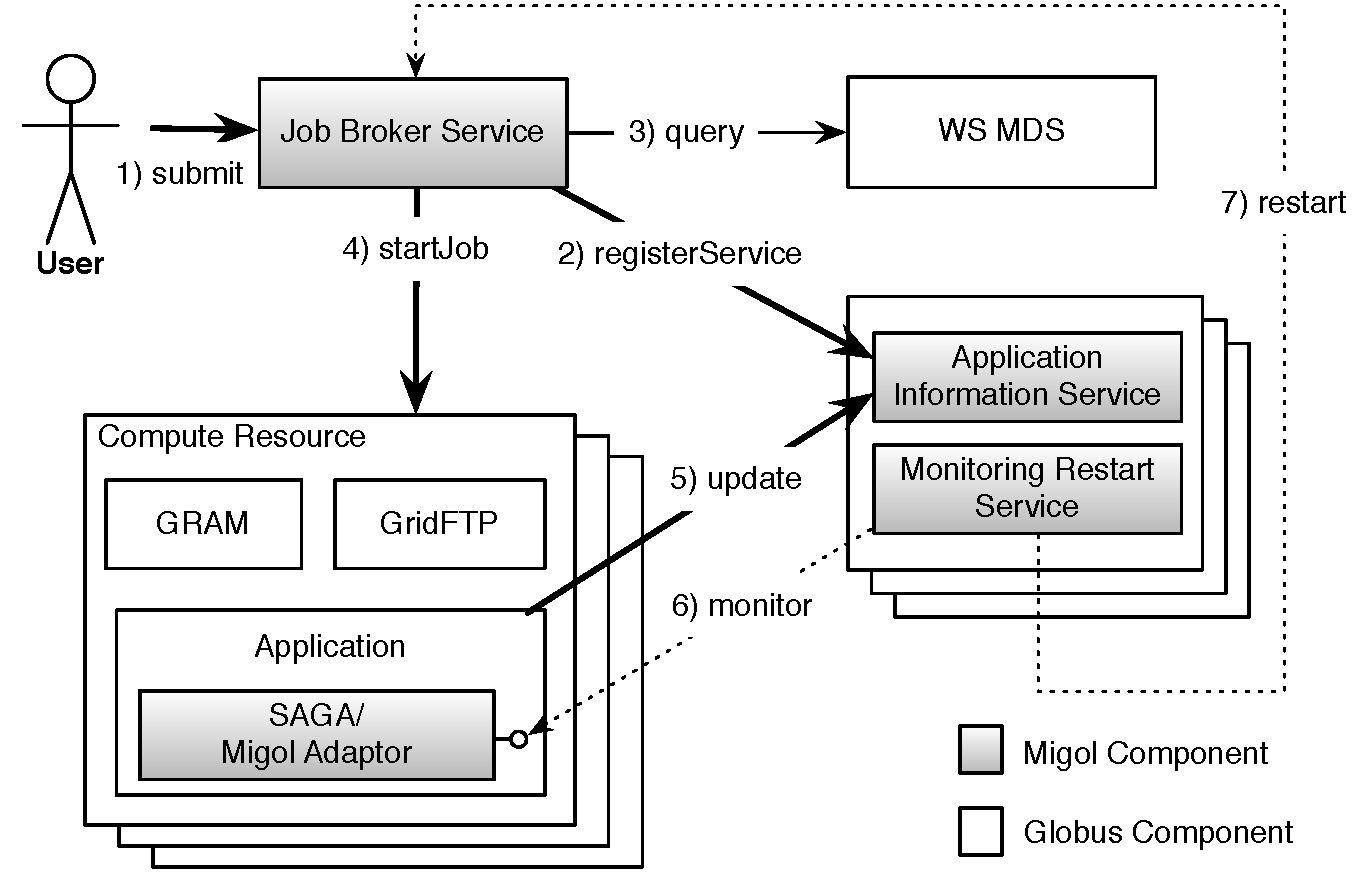
\includegraphics[width=0.9\textwidth]{migol_architecture}
%  \caption{\footnotesize \bf Migol Architecture: Migol provides
%    services for supporting the fault tolerance of Grid
%    applications. Applications that are managed by Migol are
%    transparently monitored and recovered in case of failures. }
%  \label{fig:migol_architecture} 
% \end{figure}           

% \jhanote{The fundamental metadata model of Migol is the \emph{Grid
%     Service Object (GSO)} schema, which defines a generic and
%   extensible information model for describing Grid applications.  A
%   GSO stores all relevant information about an application: resource
%   requirements, the location of binaries and checkpoint files, global
%   unique identifier (GUID), etc.  Grid Service Objects containing the
%   metadata of all running applications are stored in the {\em
%     Application Information Service (AIS)}.  To avoid a single point
%   of failure, the AIS is replicated using a ring-based replication
%   protocol, which ensures the data consistency
%   (see~\citep{Luckow:2008ys} for details).  Applications are started
%   via the {\em Job Broker Service (JBS)} (step 1,
%   Figure~\ref{fig:migol_architecture}). Before job submission, the JBS
%   must register the GSO of the application at the AIS (step 2).
%   Resource discovery is performed through WS MDS~\citep{schopf06}
%   (step 3), which aggregates data of different services, e.\,g.\ the
%   Network Weather Service (NWS)~\citep{NWS99}.  Available resources
%   are matched by the JBS according to the application
%   requirements. For execution of the application on Grid resources,
%   the JBS relies on a custom module, the Advance Reservation Service,
%   which is also capable of supporting resource reservation on top of
%   GRAM.}

% \jhanote{To detect failures, the \emph{Monitoring and Restart Service
%     (MRS)} periodically monitors all services registered at the AIS
%   (step 6).  In case the MRS discovers an inactive application, it
%   initiates a restart respectively a migration using the JBS (step 7).

\section{Challenges of Implementing Replica Exchange in Distributed
  Environments}
\label{sec:challenges}
\jhanote{Outline all the challenges: RE is loosely coupled, but there
  is a synchronization point. This leads to load-balancing and
  scheduling issues even on a single machine. However when used on
  multiple machines the scheduling issues are aggravated, ie a single
  overloaded resource or delays in passing through the scheduler can
  be a performance drain.}                
                                               

% Programming abstraction
Implementing a REMD application that is capable of running in a heterogeneous and 
raven distributed environment is a complex task. REMD involves the parallel orchestration of 
many replica jobs. To master this complexity, a well-defined programing
abstraction, that allows the scientist to focus on the application, while
having a sophisticated middleware that provides critical services, such as reliable 
job management and monitoring, is required.  

% Synchronization
Despite their mostly loosely coupled nature, REMD simulations require a small level of coupling. 
The central master, the REMD-Manager, must periodically obtain the results, i.\,e.\ the energy levels,
of all replicas to determine the new configuration of the next REMD step. 
As result of this synchronization,  a single overloaded or slow machine can delay the overall
progress. This significantly limits the  applicability of REMD 
to heterogenous distributed environments, such as Grids.
Even on a single machine the required synchronization leads to various load-balancing 
and scheduling issues. In distributed environments additional unpredictable delays
can occur, e.\,g.\  due to the required queueing of replica jobs at the local
resource management system. Such delays can have a severe impact on the overall time to completion. 
                 
% Fault Tolerance
Another important issue in error-prone distributed environment is fault tolerance. 
Especially REMD simulations are very fragile: the loss of a single replica process due to a node 
or network failure usually causes the abort of the entire simulations. Thus, 
the middleware must detect and resolve failures accurately.
                                                                
% Another challenge in a heterogeneous environments is the synchronization required after each round. In particular,
% when running REMD across multiple clusters the effects of queue wait times can be severe. To avoid this issue,
% a middleware must provide efficient mechanisms to allocate resources for multiple replica runs in a row.

\section{Implementing Distributed Replica-Exchange Using SAGA}

\jhanote{this is an important section. we need to put in details of
  how our implementation addresses issues of bigjob/smalljob to
  overcome restarting one one machine and how we overcome slowdown due
  to different scheduler loads on different machines..}

The \emph{Simple API for Grid Applications (SAGA)}~\citep{saga_gfd90}
provides an easy-to-use standardised API for developing a broad range
of distributed applications, including, but not limited to
loosely-coupled data and/or pleasingly-distributed applications.  
In particular, SAGA offers an API for the management of
checkpoint-recoverable jobs and file transfers that can be used over
heterogenous distributed environment. Thus, SAGA is ideally suited for
encoding the orchestration logic of RE simulations.

\jhanote{Joohyun: Put in a paragraph or two of the main points of the
  how it is done here; maybe even discussing the ideas related to
  checkpointing, new jobs, MPI issues discussed etc. etc. Try to
  establish what is specific to the SAGA way of doing things from what
  is a general distributed computing problem/issue}
          
\subsection{REMD-Manager Architecture}
\begin{figure}[t]
      \centering
          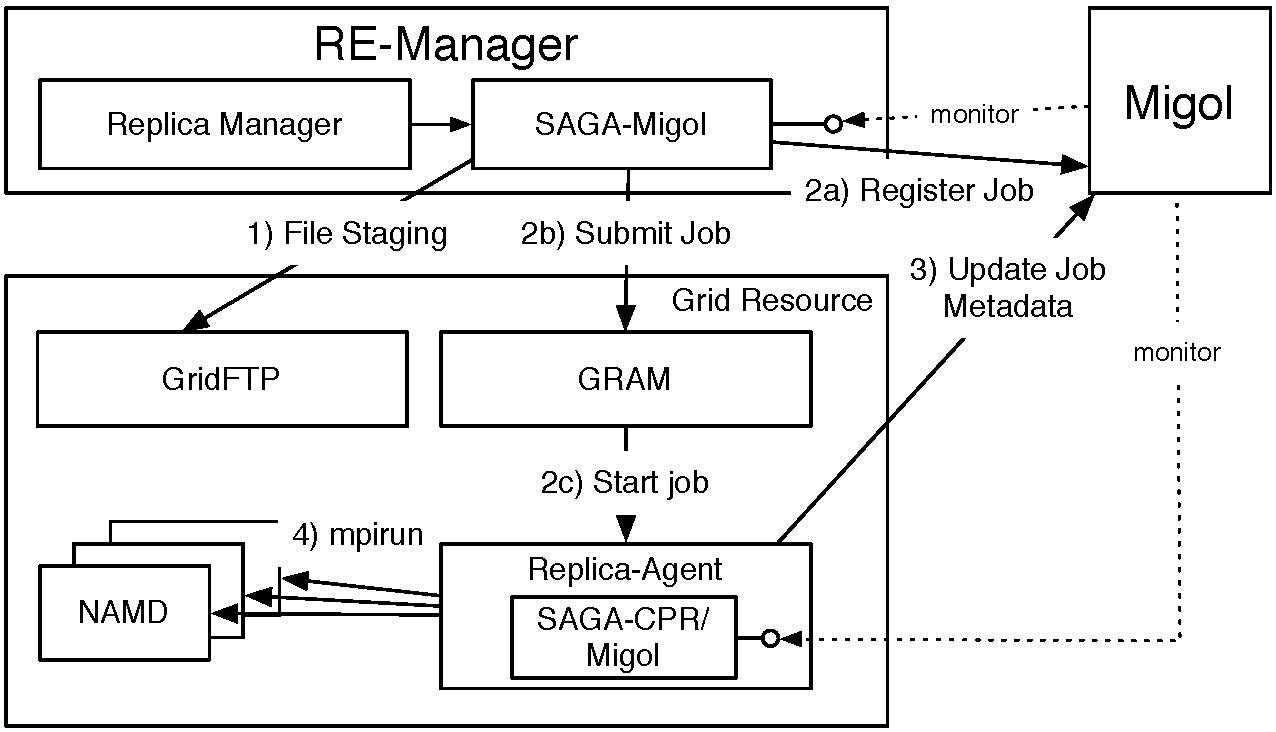
\includegraphics[width=0.7\textwidth]{REMDgManager-architecture.pdf}
          \caption{\footnotesize \bf Components of REMD-Manager: The
            main part of the framework is the replica manager. The
            manager orchestrates a set of replica processes using the
            SAGA/CPR API. The Migol infrastructure ensures that the
            REMD-Manager and all replica processes are monitored and
            recovered if necessary.}
      \label{fig:REMD-Manager-architecture}
\end{figure}

As illustrated in Figure~\ref{fig:REMD-Manager-architecture}, the
proposed framework comprises of three components: The task manager,
also referred to as \emph{REMD-Manager}, is deployed on the user's
desktop and provides the user interface to the overall REMD run. The
second component is the Migol infrastructure that submits, monitors,
and if required, recovers replica simulations.  The last element is
the task agent, the \emph{Replica-Launcher}, that resides on the High
Performance machines where MD simulations are carried out. The
NAMD-Launcher is triggered by the Grid job and is responsible for
spawning and monitoring the MD run. NAMD~\citep{Phillips:2005gd}, a
highly scalable, parallel MD code, is used to carry out the MD
simulation corresponding to each replica run. It is important to
mention that any other MD code could be used just as simply and
effectively.

The \emph{REMD-Manager} is at the core of the framework; it
orchestrates all replicas, i.\,e.\ the parameterization of replica
tasks, file staging, job spawning and the conduction of the
replica-exchange itself. This component heavily relies on the SAGA
File and CPR API as well as the Python bindings for the implementation
of the RE logic\footnote{The complete REMD-Manager code can be found
at https://svn.cct.lsu.edu/repos/saga-projects/applications/REMDgManager/}.
                                  
% \alnote{I am really not sure about this code snippet. It somehow
%   represents the logics - however I am not sure whether it is worth
%   the space.} \jhanote{I agree, that as written it is not very
%   effective. Also, since it does not show the exchange and thus the
%   reader does not see how ``distributed'' and ``local'' exchanges are
%   handled equally simply. Can we i) use psuedo-code to highlight this?
%   ii) mention where the reader can get the actually code?. We should
%   definitely do point ii) and possibly point i)}

Depending on the number of configured processes $n$, the REMD-Manager
starts $\frac{n}{2}$ pairs of replicas.  Each replica process is
assigned a different temperature. Before launching a job the
REMD-Manager ensures that all required input files are transfered to
the respective resource. For this purpose, the SAGA File API and the
GridFTP adaptor (step 1 in Figure~\ref{fig:REMD-Manager-architecture})
are used.  The replica job is then submitted to the Grid resource
using the CPR API and Migol/GRAM (step 2a-2c). Migol ensures that the
the job description of each replica is stored within the Migol backend
to ensure a later recovery. Globus GRAM is used to start the
application.

When all replicas reach a pre-determined states (e.\,g., the NAMD job finishes 
after a fixed number of steps), the decision as to whether to exchange
paired-replicas is determined by the Metropolis scheme. If successful,
parameters such as the temperature, are swapped. Both jobs are then
relaunched using the mechanisms described above. Often the Metropolis
scheme returns a negative result, and an exchange is not carried out;
thus it is difficult to respond to a possible exchange speculatively. 

           
\subsection{Efficient Replica Job Scheduling}

A particular problem that became evident in earlier
experiments~\citep{Luckow:2008la} is the effect of the 
queuing delay on the overall time to completion of a REMD run.
As state in section~\ref{sec:challenges}, REMD requires some
synchronizations after each replica round. Especially when running
REMD across multiple resources, a single crowded resource is able to
delay the completion of the simulation arbitrary. 

A common pattern to solve this issue is the usage of a meta-job, which represents
a placeholder for many small jobs. For the big meta-job a large chunk of resources 
is requested from the local resource management system. The application can then rapidly 
execute small jobs through this meta-job. By avoiding the high initial costs of queueing a job
the completion times of loosely coupled applications consisting of
many small jobs, such as the REMD-Manager, can be dramatically reduced. This principle is also known as \glidein.

Different systems that use similar approaches have been developed. \citet{citeulike:291860} initially proposed
this idea in their work on Condor Glide-In. Using Condor Glide-In a complete Condor pool can
be initiated using the GRAM service. Falkon~\citet{1362680} is a newer system, which emphasize in particular
the performance of its task dispatcher.   However, both systems have 
limitations and impose e.\,g.\ different overheads:
Condor \glidein requires the start of a complete set of Condor daemons within the
allocated set of resources. For Falcon, \citet{citeulike:3169002}
noted a startup time of over 2 minutes on a Blue Gene/P machine. Further, 
firewall issues have been reported by both systems.
  
\begin{figure}[th]
    \centering
    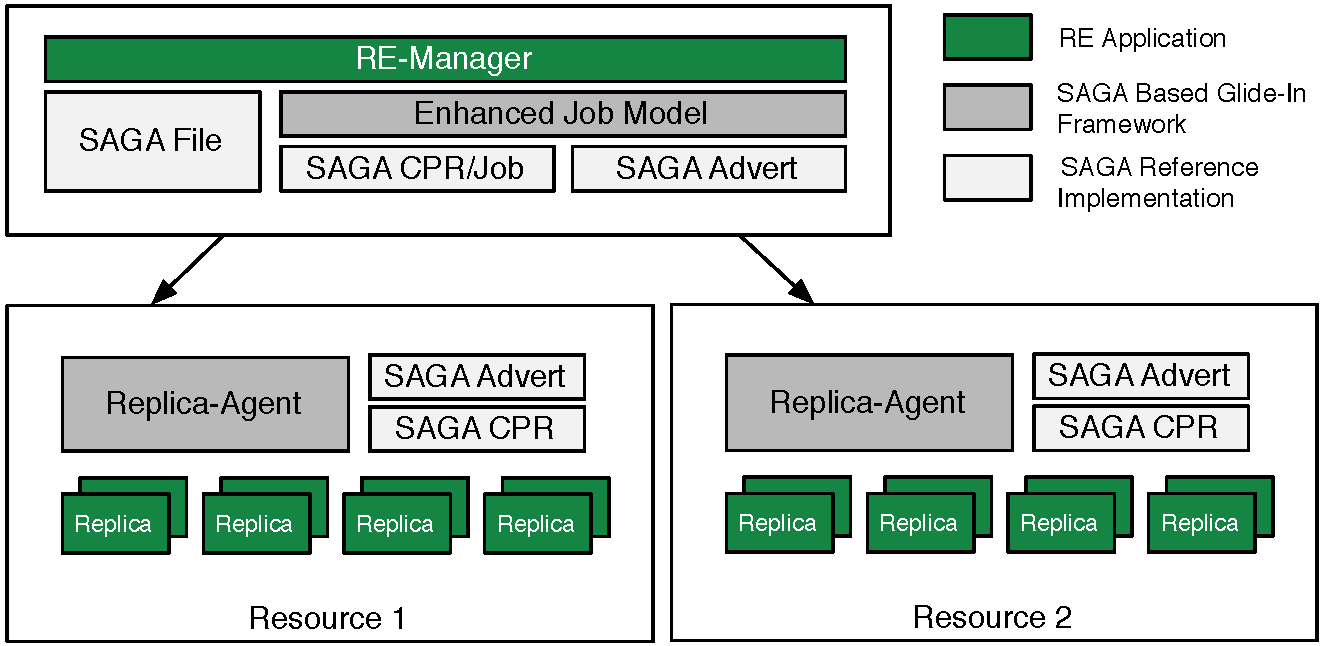
\includegraphics[width=0.9\textwidth]{remdmanager_v11}
    \caption{\footnotesize \bf REMD Programing Abstractions and
      Resource Management: The Replica-Agent is used as meta-job
      for all replica sub-jobs running on a single cluster. The
      REMD-Manager can control both the \replicaagent\ and the
      replica jobs using a SAGA-based user-level job API. By using this efficient
      way to allocate resources, queuing times are minimized and the
      time to completion can be dramatically reduced.}
    \label{fig:remdmanager_v1.1}
\end{figure}

In the following, we demonstrated the simplicity and extensibility of the SAGA framework by providing a
well-defined abstraction for \glidein based applications. This abstraction is entirely implemented
on user-level using the SAGA primitives.
Figure~\ref{fig:remdmanager_v1.1} illustrates the architecture. 
The framework comprises of three components: the REMD application itself,
the \glidein\ framework and the core SAGA system.
        
The SAGA \glidein\ framework enhances the job model of SAGA by the capability to allocate
larger chunks of resources prior to a loosely coupled run. The REMD-Manager uses
this functionality to reserve resources for all replica processes on the respective machine.
When an application requests such an allocation, the frameworks submits a meta-job,
the \textit{\replicaagent} job to the respective resource  using
the SAGA CPR API. This agent is assigned the resources required for
all replica processes on this machine. 

In the following, the REMD-Manager can rapidly execute small replica jobs using the 
enhanced Job API. For every replica job the reference
to the \replicaagent\  job id must be provided. In a sense the resources 
managed by \replicaagent\ represents a resource reservation 
and the agent represents a user-level resource manager: It is the 
responsibility of the \replicaagent\  to assign resources to
these ``small'' tasks and free these resources after completion. Further, 
the \replicaagent\ monitors all sub-jobs and registers required information with the Migol backend.


\jhanote{Let us reach consistency on, BigJob/LittleJob vs MetaJob vs
  Enhanced Job terminology}

% The enhanced job model behaves similar to the SAGA Job API. 
% The handling of such jobs is exactly the same as with the normal SAGA jobs. 

The implementation of this API is done entirely in application space using Python and
the SAGA CPR and Advert API. Using the Python duck typing mechanism such an
enhanced job object can be used as replacement to a SAGA job object --
no further source modifications needed. The implementation is based on
a simple protocol using the Advert Service, a central key/value store.
For each new job an advert entry is created. The \replicaagent\
periodically polls for new jobs.  If a new job is found and resources
are available, the job is launched otherwise it is queued.

\subsection{Reliability}
                                                                
The \replicaagent\ acts as a client for the Migol
backend. It is responsible for updating the metadata of the
application, i.\,e.\ the state, monitoring endpoint and new checkpoint
URLs, at the Migol backend. During the entire runtime the replica
process is monitored by Migol using the monitoring endpoint of the
Replica-Agent.
                           

% To integrate NAMD with the SAGA/Migol infrastructure a SAGA based task
% agent -- {\it Replica-Launcher}, is used.  This agent is responsible for
% updating the metadata of the application, i.\,e.\ the state,
% monitoring endpoint and new checkpoint URLs, at the
% Migol backend.  The agent then launches the actual NAMD job using
% MPI. During the entire runtime the replica process is monitored by
% Migol using the monitoring endpoint of the Replica-Launcher. This
% Replica-Launcher enables the flexible orchestration of multiple NAMD jobs
% through the REMD-Manager without modification of the NAMD source
% itself.    This
% Replica-Launcher enables the flexible orchestration of multiple NAMD jobs
% through the REMD-Manager without modification of the NAMD source
% itself.
               
\subsection{Conclusion}
In summary, SAGA allows the simple decoupling of the REMD application
and orchestration logic from the underlying distributed
infrastructure. All this whilst remaining general purpose and
extensible, for example, using the Migol adaptor, the application can
also benefit from additional features, such as the automatic
monitoring and the transparent recovery of failed tasks. By only
slightly extending the Job abstraction defined by SAGA a powerful
system-level abstraction such as \glidein\ jobs has been defined and
successfully deployed within the REMD application. While the current
implementation used a custom protocol to implement this mechanism, the
approach can also be applied to other middleware platforms, such as
Condor Glidin or Falcon. Currently, we are actively working on a
Condor adaptor for SAGA, which will also support native \glidein\
functionality for Condor Jobs; our implementation of \glidein\ will
then serve as a meta \glidein\, with condor level \glidein\ being usable
where appropriate.
% thus highlighting the power of programatic interface working on condor
% adaptor we could easily map this to condor \glidein
{\bf This is the first known instance of creating a system
  (deployment) level abstraction from basic programming interfaces.}


% \jhanote{May want to replace or remove: At the same time, SAGA allows
%   the application to easily utilize other infrastructures in
%   conjunction to or as replacement to Migol.}

\jhanote{We need to reference the challenges outlined in the previous
  section explicitly and mention how we have addressed them}

\section{Experiences with REMD}
\label{sec:exp}       
        
To evaluate the performance of the REMD-Manager several
experiments have been conducted on the LONI
Grid~\citep{loni}. The REMD-Manager is used to deploy tasks to
the LONI clusters: QueenBee (QB), Poseidon and Eric.  \jhanote{I think
  we want to say REMD simulations have been deployed on three LONI
  Linux Clusters? Not the managers themselves -- which I think sits on
  users desktop...}  \alnote{adjusted that - should i change figure 4
  too, although for the measurements all jobs have been launched from
  QB. There are some firewalls which limit the desktop experience.}
QB, which is both a LONI and a TeraGrid resource, is the largest LONI
machine and has a peak performance of over 50 TFlops.
Figure~\ref{fig:saga-taskfarming} gives an overview of the testbed.

\begin{figure}[t]
    \centering
        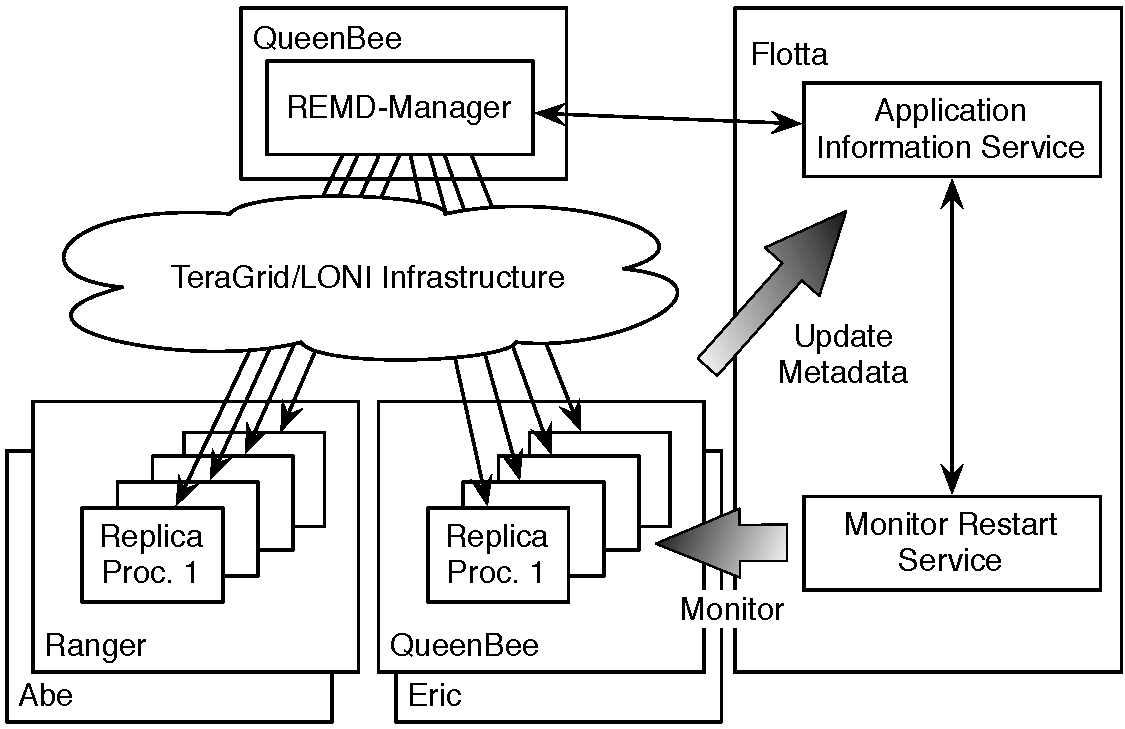
\includegraphics[width=0.7\textwidth]{saga-taskfarming}
        \caption{\footnotesize \bf Fault-Tolerant MD Simulations: The
          REMD-Manager orchestrates a set of distributed replica
          processes using the SAGA API. All processes synchronize
          important metadata with the Migol infrastructure. Migol then
          actively monitors all processes and ensures that, even in
          the presence of failures, all task are eventually
          completed.}
    \label{fig:saga-taskfarming}
\end{figure} 
The objective of the first set of experiments is the
quantification of the runtime overhead, which Migol-enabled
applications, such as the REMD-Manager encounter.  Further, we investigate the 
overall run-time reduction that can be obtained by the \replicaagent\ \glidein\
mechanism. Scientific results obtained from using this infrastructure will be reported elsewhere.
    

\subsection{Infrastructure Performance}
\begin{figure}[ht]
    \centering
        \subfloat[Submission Overhead]{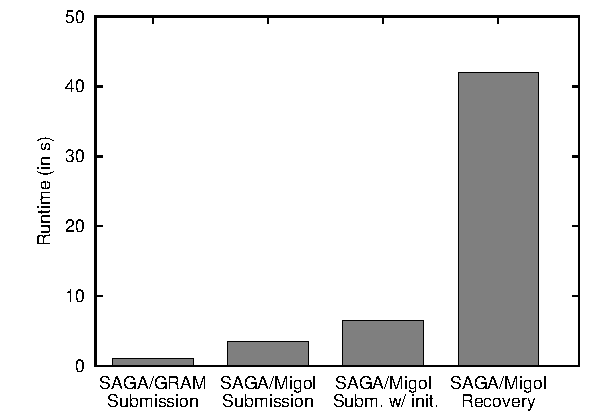
\includegraphics[width=0.48\textwidth]{performance/perf_submission.pdf} }
        \subfloat[Runtime Overhead]{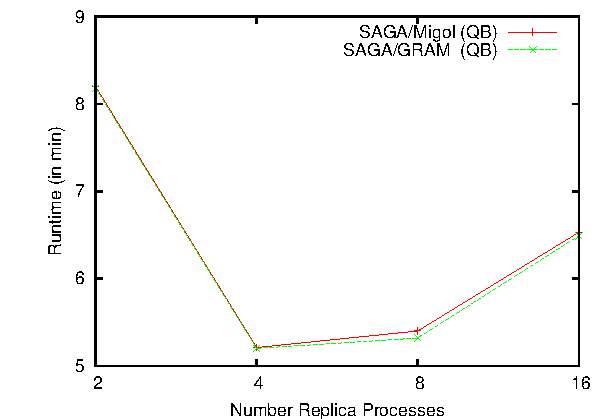
\includegraphics[width=0.49\textwidth]{performance/perf_remd.pdf} }          
    \caption{\footnotesize \bf SAGA-CPR Migol Adaptor Overhead: While the submission of Migol jobs incurs some overhead, in a real REMD scenario this overhead is negligible.}       
    \label{fig:performance_perf_submission}
\end{figure}           

Figure~\ref{fig:performance_perf_submission} shows the response-times
of SAGA-CPR submissions in comparison to their non fault-tolerant
counterparts. Since each replica exchange step involves the
relaunching of two replica jobs, the efficient spawning of remote
tasks is a critical operation for the REMD-Manager.

Initially, the submission time of a single NAMD task using
SAGA-CPR/Migol is assessed. The experiment showed that a CPR/Migol job
submission is on average 2\,seconds slower than a GRAM
submission. This overhead is mainly attributable to the additional
metadata registration operation at Migol's AIS. For jobs that run on
the order of hours, a couple of seconds overhead is effectively
negligible.

Further, the Migol adaptor showed some additional initialization
overhead. The overall runtime of the NAMD submission task including
the initialization was 6.5\,sec (bar 3 in
Fig.~\ref{fig:performance_perf_submission}), about 4.5\,sec slower
than the GRAM submission task. This overhead can be attributed to the
initialization operations for setting up the HTTP server as well as
the conduction of several metadata updates on the AIS. Since this
initialization only occurs once after the startup of the REMD-Manager,
this overhead is acceptable.
                                                                                                                    
% In addition, we investigated how the runtime of a single replica run
% is effected by Migol's active monitoring mechanism and the required
% checkpoint registration. For this purpose, a medium-size NAMD job was
% started with and without Migol support.  Monitoring intervals between
% 20\,s and 2\,minutes were chosen to study the effect of monitoring
% frequency on runtimes. The update interval for checkpoint metadata was
% set to five minutes.  Since the time measured for a checkpoint update
% operation was on average 1.3\,seconds, we do not expect this to be a
% critical factor.  The runtime of the NAMD job on QB without CPR/Migol
% amounted to 21.3 minutes.  At worst a 1 minute overhead was observable
% with a monitoring interval of 20\,s. With lower monitoring intervals,
% overheads were reduced further, e.g., the runtime overhead with a
% 2\,minute monitoring interval was only 10\,s, which is only slightly
% higher than the variance of typical NAMD runtimes. 

\subsection{REMD-Manager Performance}        

Further, we evaluated the runtime of the REMD-Manager with respect to the 
used job scheduling mechanism. The REMD-Manager was configured to run 
a simulation with 2 to 8 replica processes and 16 replica-exchange steps. 
Table~\ref{tab:app_stats} summarizes the REMD configuration used. 

% The runtime of a REMD simulation depends to a great extend on
% the queuing time at the local resource management system. Thus, we attempted 
% to minimize the queueing times during our experiment. However, as the results 
% show, small queueing delays could not always be avoided.

\jhanote{table will need updating}

\begin{table}
    \centering
	\begin{tabular}{|p{5cm}|l|}
          \hline
          %Molecular Dynamics Code &NAMD\\ \hline
          Number of NAMD steps &500\\ \hline 
          Number of MPI processes per NAMD run &16\\ \hline 
          Required staging files/size &6\,files/10\,MByte\\ \hline
          %Runtime of a single NAMD task (QB) &2\,minutes\\ \hline   
          Number of replica processes &2-64 \\ \hline   
          Temperature range (w/ 64 processes) &300 - 930 K \alnote{Joohyun: does this make sense?} \\ \hline
          Number of attempted replica-exchanges \jhanote{See caption for Q} &100\\ \hline
          %Total Runtime: &??   \\ \hline
	\end{tabular}
	\caption{\footnotesize \bf REMD Application Characteristics\label{tab:app_stats}
          \jhanote{Is 1000 the the total number of exchanges or the
            number of exchanges that a single replica will undergo?}
          For completeness we should probably mention the temperature
          range over which simulations were performed}
          \alnote{Each replica process (NAMD simulation) will conduct 
          100 steps (referred to as NAMD steps in the table). This 
          will be repeated 10 times (number exchange steps) with 
          different temperatures.}         
          \alnote{Maybe we should remove this table and put the not mentioned information 
          into the text}
          
\end{table}  
 
\begin{figure}[ht]
    \centering
    \hspace*{-20pt}
        %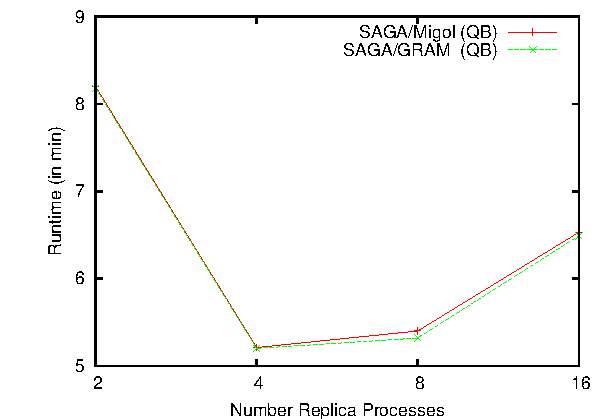
\includegraphics[width=0.5\textwidth]{performance/perf_remd.pdf}
        \caption{\footnotesize \bf REMD Runtime with and without \glidein: 
         The time that it takes to complete 16 replica exchanges; 
each replica runs for 100 steps, before attempting an exchange with
the paired-replica. Although the simultaneous deployment of
          replicas across multiple resources (labels with QB/Poseidon)
          has scheduling challenges compared to the usage of a single
          cluster (scenario QB), for scenarios studied here there is a
          slight reduction in time-to-completion.
%  The overhead of the Migol is with
%         15\,seconds negligible compared to the overall
%         runtime.
          \jhanote{need some further clarity} }
    \label{fig:performance_perf_runtime}
\end{figure}     

\alnote{This must be reworked with the new results!}
Figure~\ref{fig:performance_perf_runtime} illustrate the results of
this evaluation. Since the total number of replica exchange steps
remained constant, the runtime decreases the more replica processes
are used.  With more than four replica processes a slight decrease of
the efficiency can be observed.
% This is a result of the sequential overhead which proportional 
% grows with the number of replicas: 
The more replica processes, the more dominant the sequential overhead
at the REMD-Manager becomes. To emulate the most general case, where
each exchange step requires the staging\footnote{With a sophisticated
  data management strategy this size can further be reduced} of
different files, in our setup, we staged six files with the total size
of about 10\,MB. This transfer, which required approximately 5-10\,s
on the LONI network.  Due to the small problem set computed by each
replica (only 100 NAMD steps, which require 35\,seconds computation
time on QB), this bottleneck becomes very evident. However, in more
realistic scenarios with larger problem chunks this issue will be
avoided.


On average, with all factors considered, the SAGA/Migol adaptor added
a total runtime overhead of about 15\,seconds to the
time-to-completion.  It is important to note that this does not change
significantly with either the number of replicas, number of
replica-exchanges, nor the runtime of each replica.  Thus the results
indicate that the SAGA/Migol overhead is acceptable, corroborating
earlier findings shown in
Figure~\ref{fig:performance_perf_submission}.

Figure~\ref{fig:performance_perf_runtime} also shows that our approach
can be employed to orchestrate multiple resources concurrently, as
well as different resources (QB/Poseidon/Eric) individually.  During
the coupled distributed run, one half of the processes were allocated to
the smaller machines Eric and Poseidon, while the bulk stayed on QB.  As the
number of replicas gets larger, the concurrent distributed runs have a
lower time-to-completion than when QB was used in isolation was
observed (all else being equal). However it is important to note, that
smaller machines, such as Poseidon, showed long queuing times leading
to high variance in the overall time-to-completion. This overhead is
significant for short-running tasks and less so for longer running
tasks. 

\kimnote{However, this simple scenario faces high overhead since each
  job is submitted to the local scheduler in many cases. \it Shantenu,
  may be you can write here another scenario we discussed as an
  alternative to the simple scenario we are testing.  If I can, I will
  try, too } \alnote{I added some remarks towards a enhanced scenario
  as result of the measurements}
  

Since the probability of a failure during a 10 minute run on a few
resources is rather low, the reliability of the proposed framework was
validated by introducing faults into the systems. We killed selected
replica processes and measured the time required by Migol to restart
the system.  Due to the selected monitoring interval of one minute and
failure threshold of 2 tries, the failure detection time averages to
2.5\, minutes.

As shown in Figure~\ref{fig:performance_perf_submission}, the recovery
time required for the restart of the job is $\sim42$ seconds. This is
mainly caused by the complex interactions conducted by the Migol
backend (cmp. section~\ref{sec:migol}): The monitoring service
initializes the restart at the JBS.  A major performance penalty is
the delegation-on-demand mechanism required to obtain the credential
of the user from the AIS -- this procedure demands the creation of a
public-private key pair, which is very costly. Further, the resource
discovery and selection mechanisms used by Migol's JBS are designed
with a focus on long-running applications, and currently show some
substantial overhead, especially when used for short-running tasks.


While these results show that SAGA-CPR in conjunction with Migol
incurs some overhead, we believe that this is acceptable compared to
the benefits a fault-tolerant, self-healing infrastructure offers. In
addition, it must be noted that further simple yet effective
optimizations are possible. For example, by directly restarting jobs
via the GRAM service a lot of the overhead caused by the dynamic
discovery mechanisms of the JBS can be avoided. Further, we will
evaluate possibilities to decouple the dispatching of replica runs
from allocation of cluster resources to avoid long queuing
delays. Systems, such as Falkon~\citep{1362680} or the Condor
Glide-In~\citep{citeulike:291860} mechanism provide the possibility to
acquire chunks of resources from the resource management systems,
which can then be used to dispatch short tasks. 


\section{Related Work}


\jhanote{This section should focus on both just the ``algorithmic''
  advances/modification around Replica Exchange. But also
  advances/related work around  implementation in distributed
  environments}
                       
\alnote{Should we add related work with respect to glide-in?}

\jhanote{Joohyun: can you put in information on the AREMD and other
  papers you have sent around?}


% \jhanote{This might have to be commented out: Checkpointing and
%   rollback recovery is widely used in Grids. For example, the
%   Condor/PGRADE system~\citep{DBLP:conf/eagc/KovacsK04} consists of a
%   checkpointing mechanism for PVM applications and uses
%   Condor-G~\citep{citeulike:291860} for scheduling.  While PGRADE
%   emphasises an integrated user-level checkpoint approach, we believe
%   that this approach is not suitable for a heterogeneous Grid
%   landscape. Further, the framework does not ensure the
%   fault-tolerance of the service infrastructure sufficiently.}
                                 
\jhanote{This will have to be commented out: Further, these frameworks
  or schedulers focus on individual aspects, e.\,g.\ Nimrod-G focuses
  on task farming or GridWay on meta-scheduling. Migol aims to provide
  an overall autonomic, self-healing infrastructure, which addresses
  the fault tolerance of Grid applications and the infrastructure
  itself.}

% \noindent{\it Previous CPR Efforts:} Several frameworks for
% high-throughput computing and task farming exist,
% Condor-G~\citep{citeulike:291860}, Nimrod-G~\citep{buyya00nimrodg}, and
% Legion~\citep{689541} to name a few. These provide basic fault
% tolerance support by automatic re-scheduling failed tasks. Advanced
% features such as the management of checkpoints however, are not
% supported. Further, these frameworks rely on a very simple failure
% detection mechanism -- usually by simply polling the job state at the
% Globus gatekeeper. This allows the detection of some errors, but
% application-level failure detectors as used by the Migol/SAGA library
% can detect much more complex errors. For example, especially parallel
% applications can fail quite inconsistently: in the best case the
% application aborts, at worst the application hangs indefinitely. These
% kind of failures are not visible at Grid resource management system
% level.

% At the level of related application programming interfaces for
% checkpointing, proprietary interfaces are dominant. This is because
% applications most often rely on application level checkpointing, and
% perform also their own checkpoint management (checkpointing policies,
% frequencies, dependencies, staging etc).  \alnote{Should we remove
%   this from here - this is already mentioned now at the beginning.}
% The Open Grid Forum's\footnote{\texttt{http://www.ogf.org}} GridCPR
% group (Grid CheckPoint and Recovery) made an early attempt to describe
% a generic CPR architecture, and to define a generic CPR API, which
% would support applications to manage their complete
% checkpoint/recovery life cycle~\citep{ogf_cpr_arch}.  Based on that
% architecture, and on a set of CPR use cases~\citep{ogf_cpr_uc}, the
% SAGA group in OGF defined the CPR API package~\citep{saga_cpr_draft}
% (work in progress), whose implementation is described in this paper.
% The rendering of the CPR API in the SAGA API framework allows (a) to
% seamlessly combine CPR operations and other high level Grid
% programming abstractions provided by SAGA, and (b) to abstract from
% the actual implementation of the CPR mechanism.  The CPR API which has
% been demonstrated with the Migol framework, can work as well with
% other systems, e.\,g.\, the XtreemOS system level checkpointing
% capabilities~\citep{xtreemos_cpr}.

\noindent{\it Other Distributed RE simulations:}
Several projects, such as Folding@home and WISDOM, utilise distributed
infrastructures. While
Folding@home~\citep{PhysRevLett.86.4983}\footnote{Folding@Home~\citep{PhysRevLett.86.4983}
  is parallel replica dynamics but that is a special case of
  replica-exchange; when a certain event happens, there is a need for
  coordination amongst ALL replicas. We should maybe point this out,
  but I think it is fair at this level of detail, to consider
  folding@Home to be in the same application class to effectively
  parallelize simulations} is based on BOINC~\citep{1033223}, the
WISDOM project utilizes the EGEE infrastructure. 
Although WISDOM has similar application characteristics as discussed
here, the project is currently tied to the gLite~\citep{glite}
middleware.  In contrast to WISDOM and Folding@home, our approach is
not restricted to a specific distributed environment. SAGA based
job-launching and file-handling is supported on most general-purpose
Grids via the appropriate adaptors, as SAGA is a community
specification and is soon to be standard~\citep{saga_url}

\alnote{Should we add some details regarding the scientific results of
  WISDOM and Folding@home and how they differ from our REMD with NAMD?
  Or are we just comparing the Grid infrastructure?}  \jhanote{In
  response to immediately preceeding alnote, IMHO we don't need to
  address scientific results, but will just say the ``size of the
  problem'' that can be studied is limited}

%%------------------------------------------------------------------------------
\section{Conclusion and Future Work}

\jhanote{Mention BQP and co-scheduling as opposed to opportunistic
  approach. Reference Kalman-filter work. Reference Promita's work
  using BQP for tightly-coupled applications}.

We have developed a fault-tolerant framework that implements a
commonly occurring application usage pattern: loose-coupling of
multiple tightly-coupled applications. The framework is general
purpose and extensible to different usage patterns, deployment
scenarios and specific simulation codes.

The fault-tolerant framework used to implement RE simulations in a
production environment is created using the distributed programming
interfaces provided by SAGA and its coupling to Migol.  SAGA provides
a middleware-independent, programing abstraction for distributed
environments. RE simulations utilize the new SAGA-CPR API to interface
with a checkpoint-recovery infrastructure, such as Migol. Using the
newly developed SAGA adaptor for Migol, any SAGA application can
re-use Migol's fault-tolerant services for monitoring and recovery.
The application developer is not required to provide any special code,
just the Migol adaptor must be configured.  The Migol framework has
strong self-healing capabilities: critical services, such as the
Application Information Service (AIS) are able to automatically detect
failures and reconfigure themselves, and thus addresses common failure
modes in distributed environments without user interaction.
In case of failures, e.\,g.,\ a node-crash, applications are
automatically restarted from the last saved
checkpoint.

In contrast to other RE implementations on distributed simulations, it
is critical to note and emphasise the general usability and
extensibility -- across different infrastructures, across a range of
scientific applications and usage patterns (e.g.  the multiple
variants of the RE) -- of our approach.
                  
\alnote{Gallicchio et al.: AREMD}
                                         
Future Work: 
- prefetching of tasks
- investigate different scheduling variant


\jhanote{In future work, we need to mention that we are deploying this
  infrastructure on a real distributed system (LONI) and are using it
  to study the binding interactions of peptide-RNA (Joohyun, would you
  agree?). We will report on the specific science results obtained
  using this approach in publication TBD but most likely Phil Trans of
  Royal Soc A}

\begin{acknowledgement}
   This work would not have been possible without the efforts and
  support of the wider SAGA team, especially Hartmut Kaiser, Ole
  Weidner and Joao Abecasis. We also thank Daniel Katz for hosting AL
  at the CCT, when this work was conceived.  Important funding for
  SAGA specification and development has been provided by the UK EPSRC
  grant number GR/D0766171/1 (via OMII).  SJ acknowledges the
  e-Science Institute, Edinburgh for supporting the research theme,
  ``Distributed Programming Abstractions''.  This work has also been
  made possible thanks to the internal resources of the Center for
  Computation \& Technology (CCT) at Louisiana State University and
  computer resources provided by LONI.
\end{acknowledgement}

% \begin{thebibliography}  {10}
% \bibitem{dpa-paper}
% S. Jha et al., {\em Programming Abstractions for Large-scale Distributed
%   Applications}, to be submitted to ACM Computing Surveys; draft at
%   \url{http://www.cct.lsu.edu/~sjha/publications/dpa_surveypaper.pdf}.
% \end{thebibliography}

%\bibliographystyle{IEEEtran}
\bibliographystyle{kluwer}
\bibliography{saga,literatur}    
\end{document}

